% Options for packages loaded elsewhere
\PassOptionsToPackage{unicode}{hyperref}
\PassOptionsToPackage{hyphens}{url}
\PassOptionsToPackage{dvipsnames,svgnames,x11names}{xcolor}
%
\documentclass[
  letterpaper,
  DIV=11,
  numbers=noendperiod]{scrartcl}

\usepackage{amsmath,amssymb}
\usepackage{lmodern}
\usepackage{iftex}
\ifPDFTeX
  \usepackage[T1]{fontenc}
  \usepackage[utf8]{inputenc}
  \usepackage{textcomp} % provide euro and other symbols
\else % if luatex or xetex
  \usepackage{unicode-math}
  \defaultfontfeatures{Scale=MatchLowercase}
  \defaultfontfeatures[\rmfamily]{Ligatures=TeX,Scale=1}
\fi
% Use upquote if available, for straight quotes in verbatim environments
\IfFileExists{upquote.sty}{\usepackage{upquote}}{}
\IfFileExists{microtype.sty}{% use microtype if available
  \usepackage[]{microtype}
  \UseMicrotypeSet[protrusion]{basicmath} % disable protrusion for tt fonts
}{}
\makeatletter
\@ifundefined{KOMAClassName}{% if non-KOMA class
  \IfFileExists{parskip.sty}{%
    \usepackage{parskip}
  }{% else
    \setlength{\parindent}{0pt}
    \setlength{\parskip}{6pt plus 2pt minus 1pt}}
}{% if KOMA class
  \KOMAoptions{parskip=half}}
\makeatother
\usepackage{xcolor}
\setlength{\emergencystretch}{3em} % prevent overfull lines
\setcounter{secnumdepth}{-\maxdimen} % remove section numbering
% Make \paragraph and \subparagraph free-standing
\ifx\paragraph\undefined\else
  \let\oldparagraph\paragraph
  \renewcommand{\paragraph}[1]{\oldparagraph{#1}\mbox{}}
\fi
\ifx\subparagraph\undefined\else
  \let\oldsubparagraph\subparagraph
  \renewcommand{\subparagraph}[1]{\oldsubparagraph{#1}\mbox{}}
\fi

\usepackage{color}
\usepackage{fancyvrb}
\newcommand{\VerbBar}{|}
\newcommand{\VERB}{\Verb[commandchars=\\\{\}]}
\DefineVerbatimEnvironment{Highlighting}{Verbatim}{commandchars=\\\{\}}
% Add ',fontsize=\small' for more characters per line
\usepackage{framed}
\definecolor{shadecolor}{RGB}{241,243,245}
\newenvironment{Shaded}{\begin{snugshade}}{\end{snugshade}}
\newcommand{\AlertTok}[1]{\textcolor[rgb]{0.68,0.00,0.00}{#1}}
\newcommand{\AnnotationTok}[1]{\textcolor[rgb]{0.37,0.37,0.37}{#1}}
\newcommand{\AttributeTok}[1]{\textcolor[rgb]{0.40,0.45,0.13}{#1}}
\newcommand{\BaseNTok}[1]{\textcolor[rgb]{0.68,0.00,0.00}{#1}}
\newcommand{\BuiltInTok}[1]{\textcolor[rgb]{0.00,0.23,0.31}{#1}}
\newcommand{\CharTok}[1]{\textcolor[rgb]{0.13,0.47,0.30}{#1}}
\newcommand{\CommentTok}[1]{\textcolor[rgb]{0.37,0.37,0.37}{#1}}
\newcommand{\CommentVarTok}[1]{\textcolor[rgb]{0.37,0.37,0.37}{\textit{#1}}}
\newcommand{\ConstantTok}[1]{\textcolor[rgb]{0.56,0.35,0.01}{#1}}
\newcommand{\ControlFlowTok}[1]{\textcolor[rgb]{0.00,0.23,0.31}{#1}}
\newcommand{\DataTypeTok}[1]{\textcolor[rgb]{0.68,0.00,0.00}{#1}}
\newcommand{\DecValTok}[1]{\textcolor[rgb]{0.68,0.00,0.00}{#1}}
\newcommand{\DocumentationTok}[1]{\textcolor[rgb]{0.37,0.37,0.37}{\textit{#1}}}
\newcommand{\ErrorTok}[1]{\textcolor[rgb]{0.68,0.00,0.00}{#1}}
\newcommand{\ExtensionTok}[1]{\textcolor[rgb]{0.00,0.23,0.31}{#1}}
\newcommand{\FloatTok}[1]{\textcolor[rgb]{0.68,0.00,0.00}{#1}}
\newcommand{\FunctionTok}[1]{\textcolor[rgb]{0.28,0.35,0.67}{#1}}
\newcommand{\ImportTok}[1]{\textcolor[rgb]{0.00,0.46,0.62}{#1}}
\newcommand{\InformationTok}[1]{\textcolor[rgb]{0.37,0.37,0.37}{#1}}
\newcommand{\KeywordTok}[1]{\textcolor[rgb]{0.00,0.23,0.31}{#1}}
\newcommand{\NormalTok}[1]{\textcolor[rgb]{0.00,0.23,0.31}{#1}}
\newcommand{\OperatorTok}[1]{\textcolor[rgb]{0.37,0.37,0.37}{#1}}
\newcommand{\OtherTok}[1]{\textcolor[rgb]{0.00,0.23,0.31}{#1}}
\newcommand{\PreprocessorTok}[1]{\textcolor[rgb]{0.68,0.00,0.00}{#1}}
\newcommand{\RegionMarkerTok}[1]{\textcolor[rgb]{0.00,0.23,0.31}{#1}}
\newcommand{\SpecialCharTok}[1]{\textcolor[rgb]{0.37,0.37,0.37}{#1}}
\newcommand{\SpecialStringTok}[1]{\textcolor[rgb]{0.13,0.47,0.30}{#1}}
\newcommand{\StringTok}[1]{\textcolor[rgb]{0.13,0.47,0.30}{#1}}
\newcommand{\VariableTok}[1]{\textcolor[rgb]{0.07,0.07,0.07}{#1}}
\newcommand{\VerbatimStringTok}[1]{\textcolor[rgb]{0.13,0.47,0.30}{#1}}
\newcommand{\WarningTok}[1]{\textcolor[rgb]{0.37,0.37,0.37}{\textit{#1}}}

\providecommand{\tightlist}{%
  \setlength{\itemsep}{0pt}\setlength{\parskip}{0pt}}\usepackage{longtable,booktabs,array}
\usepackage{calc} % for calculating minipage widths
% Correct order of tables after \paragraph or \subparagraph
\usepackage{etoolbox}
\makeatletter
\patchcmd\longtable{\par}{\if@noskipsec\mbox{}\fi\par}{}{}
\makeatother
% Allow footnotes in longtable head/foot
\IfFileExists{footnotehyper.sty}{\usepackage{footnotehyper}}{\usepackage{footnote}}
\makesavenoteenv{longtable}
\usepackage{graphicx}
\makeatletter
\def\maxwidth{\ifdim\Gin@nat@width>\linewidth\linewidth\else\Gin@nat@width\fi}
\def\maxheight{\ifdim\Gin@nat@height>\textheight\textheight\else\Gin@nat@height\fi}
\makeatother
% Scale images if necessary, so that they will not overflow the page
% margins by default, and it is still possible to overwrite the defaults
% using explicit options in \includegraphics[width, height, ...]{}
\setkeys{Gin}{width=\maxwidth,height=\maxheight,keepaspectratio}
% Set default figure placement to htbp
\makeatletter
\def\fps@figure{htbp}
\makeatother

\KOMAoption{captions}{tableheading}
\makeatletter
\makeatother
\makeatletter
\makeatother
\makeatletter
\@ifpackageloaded{caption}{}{\usepackage{caption}}
\AtBeginDocument{%
\ifdefined\contentsname
  \renewcommand*\contentsname{Table of contents}
\else
  \newcommand\contentsname{Table of contents}
\fi
\ifdefined\listfigurename
  \renewcommand*\listfigurename{List of Figures}
\else
  \newcommand\listfigurename{List of Figures}
\fi
\ifdefined\listtablename
  \renewcommand*\listtablename{List of Tables}
\else
  \newcommand\listtablename{List of Tables}
\fi
\ifdefined\figurename
  \renewcommand*\figurename{Figure}
\else
  \newcommand\figurename{Figure}
\fi
\ifdefined\tablename
  \renewcommand*\tablename{Table}
\else
  \newcommand\tablename{Table}
\fi
}
\@ifpackageloaded{float}{}{\usepackage{float}}
\floatstyle{ruled}
\@ifundefined{c@chapter}{\newfloat{codelisting}{h}{lop}}{\newfloat{codelisting}{h}{lop}[chapter]}
\floatname{codelisting}{Listing}
\newcommand*\listoflistings{\listof{codelisting}{List of Listings}}
\makeatother
\makeatletter
\@ifpackageloaded{caption}{}{\usepackage{caption}}
\@ifpackageloaded{subcaption}{}{\usepackage{subcaption}}
\makeatother
\makeatletter
\@ifpackageloaded{tcolorbox}{}{\usepackage[many]{tcolorbox}}
\makeatother
\makeatletter
\@ifundefined{shadecolor}{\definecolor{shadecolor}{rgb}{.97, .97, .97}}
\makeatother
\makeatletter
\makeatother
\ifLuaTeX
  \usepackage{selnolig}  % disable illegal ligatures
\fi
\IfFileExists{bookmark.sty}{\usepackage{bookmark}}{\usepackage{hyperref}}
\IfFileExists{xurl.sty}{\usepackage{xurl}}{} % add URL line breaks if available
\urlstyle{same} % disable monospaced font for URLs
\hypersetup{
  pdftitle={Data and Information},
  colorlinks=true,
  linkcolor={blue},
  filecolor={Maroon},
  citecolor={Blue},
  urlcolor={Blue},
  pdfcreator={LaTeX via pandoc}}

\title{{Data and Information}}
\author{}
\date{}

\begin{document}
\maketitle
\ifdefined\Shaded\renewenvironment{Shaded}{\begin{tcolorbox}[interior hidden, enhanced, borderline west={3pt}{0pt}{shadecolor}, sharp corners, breakable, frame hidden, boxrule=0pt]}{\end{tcolorbox}}\fi

\hypertarget{do-we-need-study-designs-anymore-to-do-research}{%
\subsection{Do we need study designs anymore to do
research?}\label{do-we-need-study-designs-anymore-to-do-research}}

\begin{figure}

{\centering 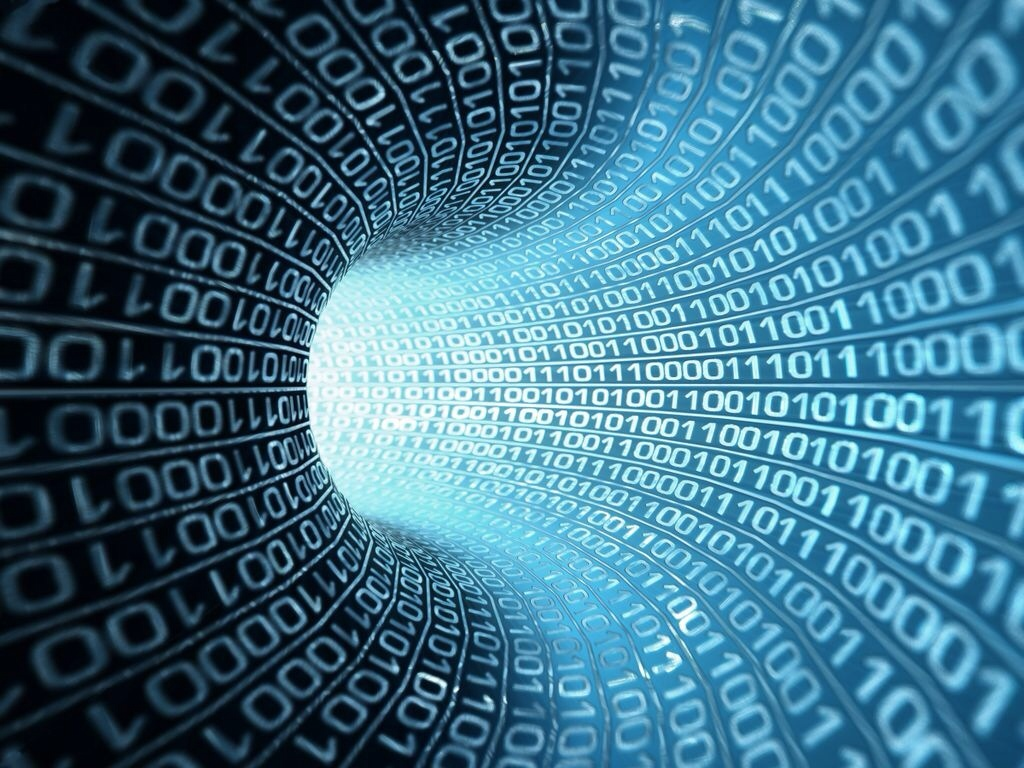
\includegraphics[width=4.88542in,height=\textheight]{Information_files/BigData.png}

}

\end{figure}

\hypertarget{big-data-problems}{%
\subsection{Big Data Problems}\label{big-data-problems}}

\href{https://hbr.org/2013/04/the-hidden-biases-in-big-data}{``\emph{The
hidden Biases of Big Data}'' by Kate Crawford}

\textbf{Harvard Business Review (2013)}

. . .

\begin{figure}

{\centering 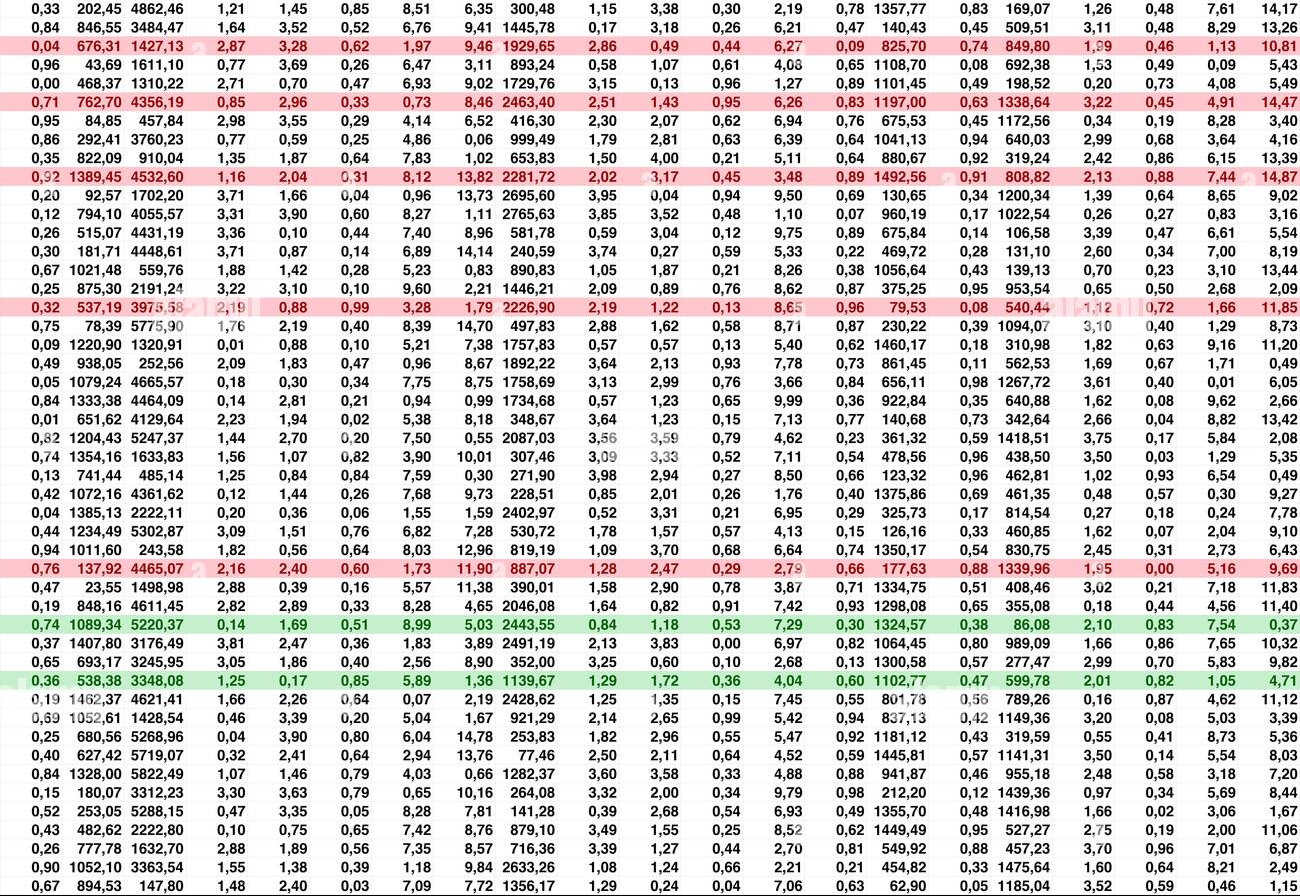
\includegraphics[width=5.20833in,height=\textheight]{Information_files/spreadsheet.png}

}

\end{figure}

\hypertarget{big-data-problems-1}{%
\subsection{Big Data Problems}\label{big-data-problems-1}}

\href{https://hbr.org/2013/04/the-hidden-biases-in-big-data}{``\emph{The
hidden Biases of Big Data}'' by Kate Crawford}

\textbf{Harvard Business Review (2013)}

. . .

\begin{figure}

{\centering 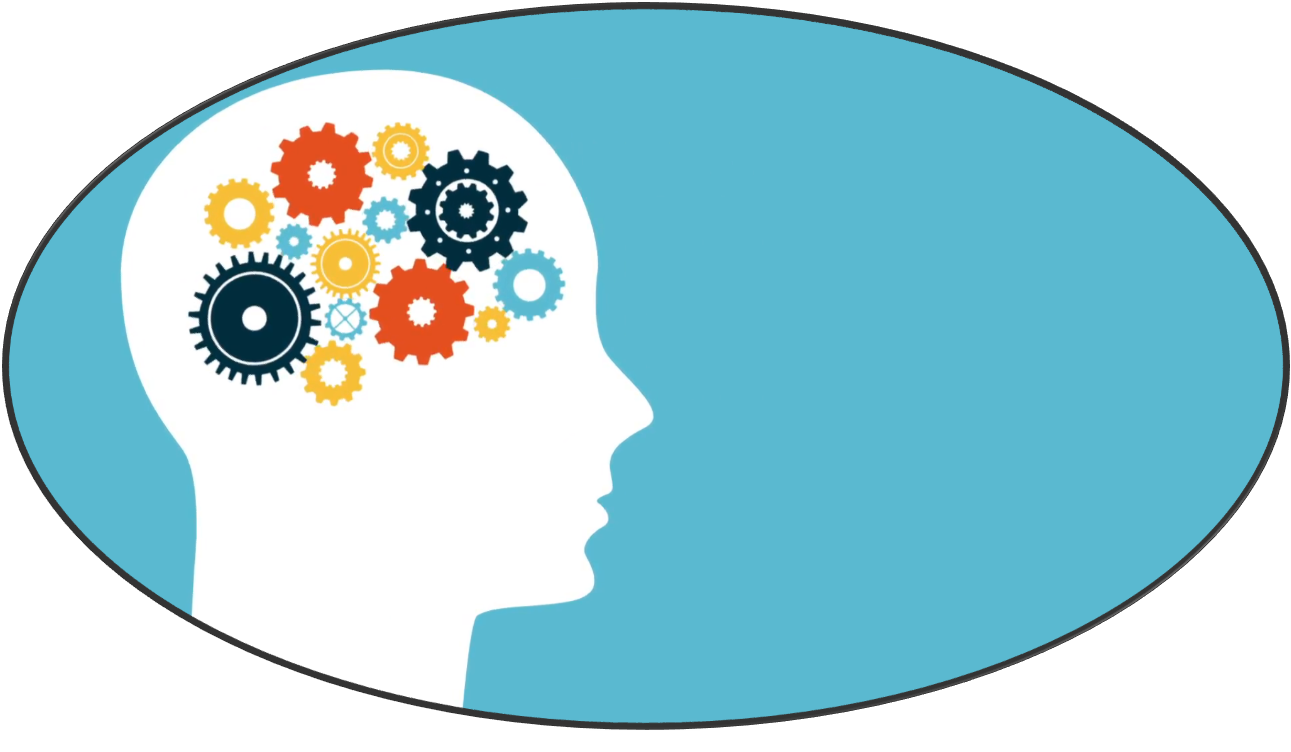
\includegraphics[width=4.78125in,height=\textheight]{Information_files/thinking.png}

}

\end{figure}

\hypertarget{big-data-problems-2}{%
\subsection{Big Data Problems}\label{big-data-problems-2}}

\href{https://projecteuclid.org/journals/annals-of-applied-statistics/volume-12/issue-2/Statistical-paradises-and-paradoxes-in-big-data-I--Law/10.1214/18-AOAS1161SF.full}{\textbf{The
Annals of Applied Statistics (2018); Xiao Li Meng,}}

. . .

. . .

Sampling Processes == Human Design

. . .

\textbf{What is worse?}

\begin{itemize}
\tightlist
\item
  a very precise inaccurate result
\item
  an accurate imprecise result
\end{itemize}

\hypertarget{big-data-problems-3}{%
\subsection{Big Data Problems}\label{big-data-problems-3}}

\begin{figure}

{\centering 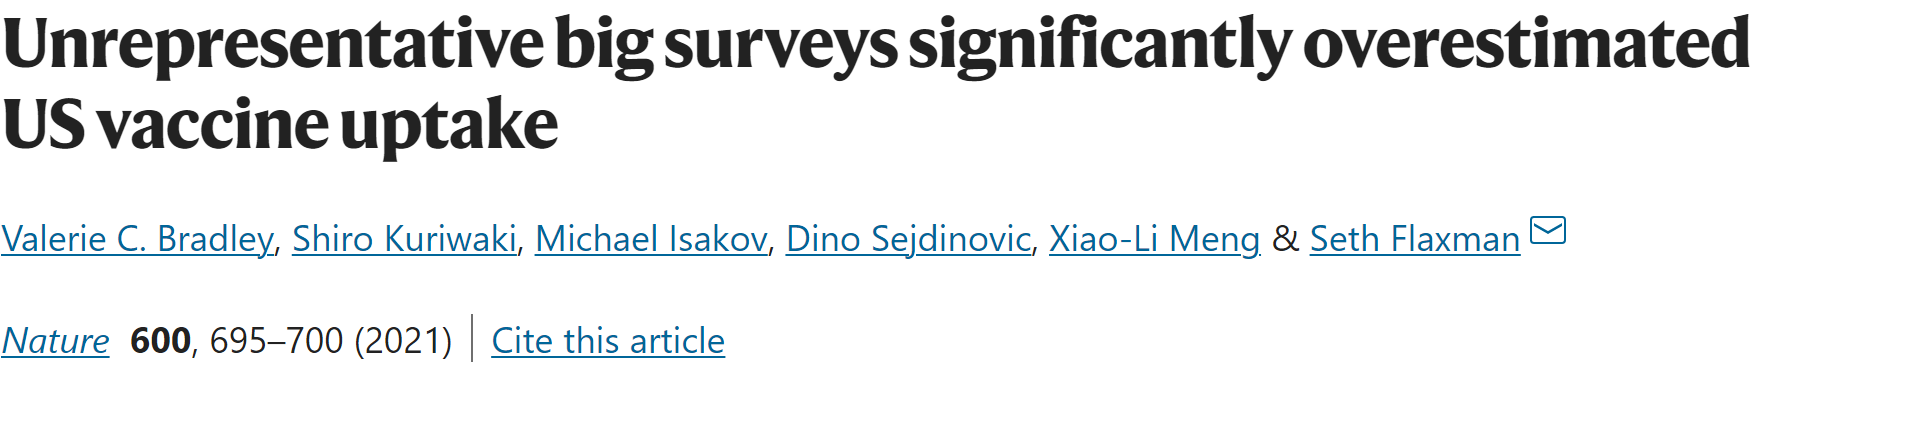
\includegraphics[width=10.41667in,height=\textheight]{Information_files/survey.data.png}

}

\caption{\href{https://www.nature.com/articles/s41586-021-04198-4}{link}}

\end{figure}

. . .

\hypertarget{big-data-problems-4}{%
\subsection{Big Data Problems}\label{big-data-problems-4}}

Using eBird data w/o accounting for sampling biases.

. . .

\begin{figure}

{\centering 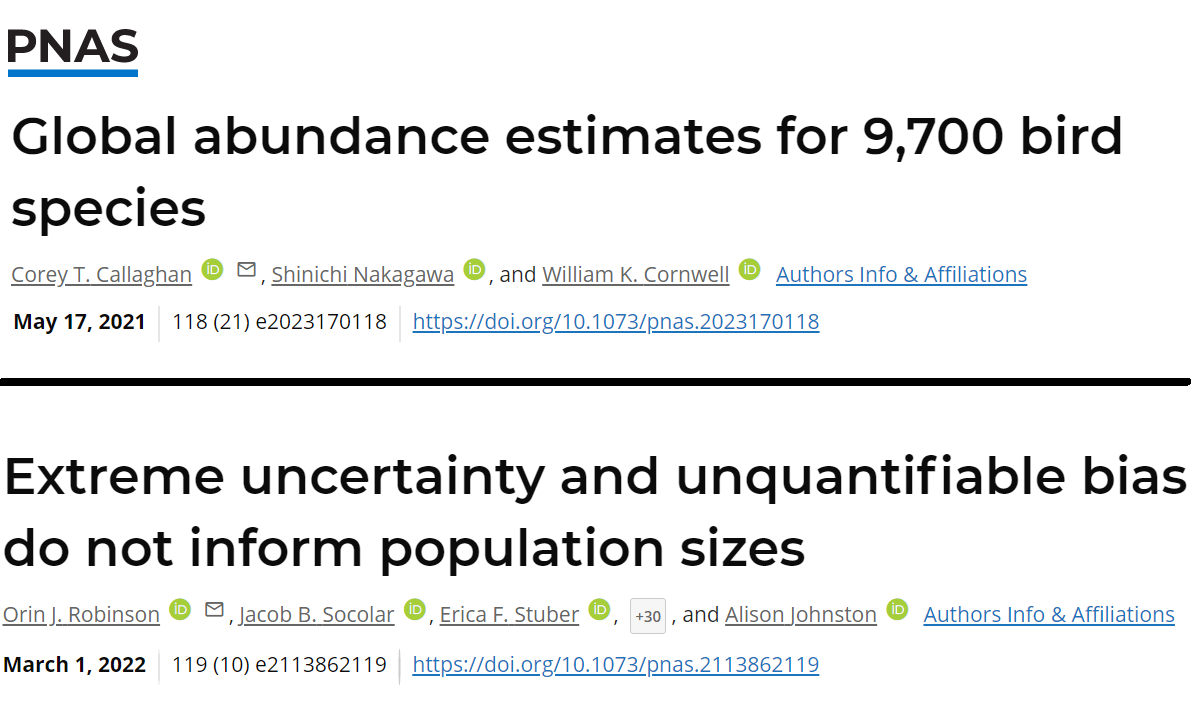
\includegraphics{Information_files/ebird.png}

}

\end{figure}

\href{https://www.pnas.org/doi/10.1073/pnas.2023170118}{Link1}.
\href{https://www.pnas.org/doi/10.1073/pnas.2113862119}{Link2}.

. . .

. . .

\hypertarget{the-questioning-scientist}{%
\subsection{The Questioning Scientist}\label{the-questioning-scientist}}

In regard to \emph{data} and \emph{statistical models},
{21\textsuperscript{st} century scientists should be pragmatic, excited,
and questioning.}

\begin{itemize}
\tightlist
\item
  How and why did these data come to be?

  \begin{itemize}
  \tightlist
  \item
    \emph{understand the study design}
  \item
    \emph{ask this even when you design the study, after data
    collection}
  \end{itemize}
\end{itemize}

\begin{itemize}
\tightlist
\item
  What do these data look like?

  \begin{itemize}
  \tightlist
  \item
    \emph{visualize the data in many dimensions}
  \item
    \emph{keep in mind - not all outcomes are visible in data --
    example?}
  \end{itemize}
\end{itemize}

\begin{itemize}
\tightlist
\item
  How does this statistical model work?

  \begin{itemize}
  \tightlist
  \item
    \emph{statistical notation, explicit and implicit assumptions},
    \emph{optimization}
  \end{itemize}
\end{itemize}

\begin{itemize}
\tightlist
\item
  How does this statistical model fail in theory and in practice?

  \begin{itemize}
  \tightlist
  \item
    \emph{statistical robustness and identifiability}
  \end{itemize}
\end{itemize}

\hypertarget{data-vs.-information}{%
\subsection{Data vs.~Information}\label{data-vs.-information}}

. . .

\begin{figure}

{\centering 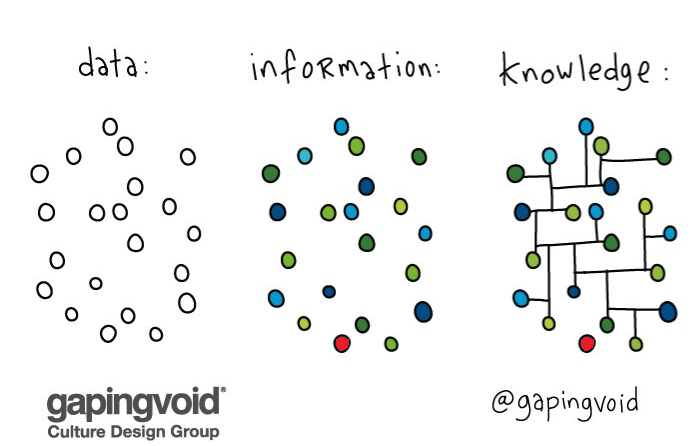
\includegraphics{Information_files/info_diagram.png}

}

\end{figure}

\hypertarget{information}{%
\subsection{Information}\label{information}}

\begin{itemize}
\tightlist
\item
  the question being asked of the data
\item
  how the data came to be
\item
  the goal of the question
\end{itemize}

\hypertarget{the-question-and-the-data}{%
\subsection{The question and the data}\label{the-question-and-the-data}}

Ecological surveillance monitoring will often have \emph{low quality
information} regarding post-hoc hypotheses.

. . .

\begin{figure}

{\centering 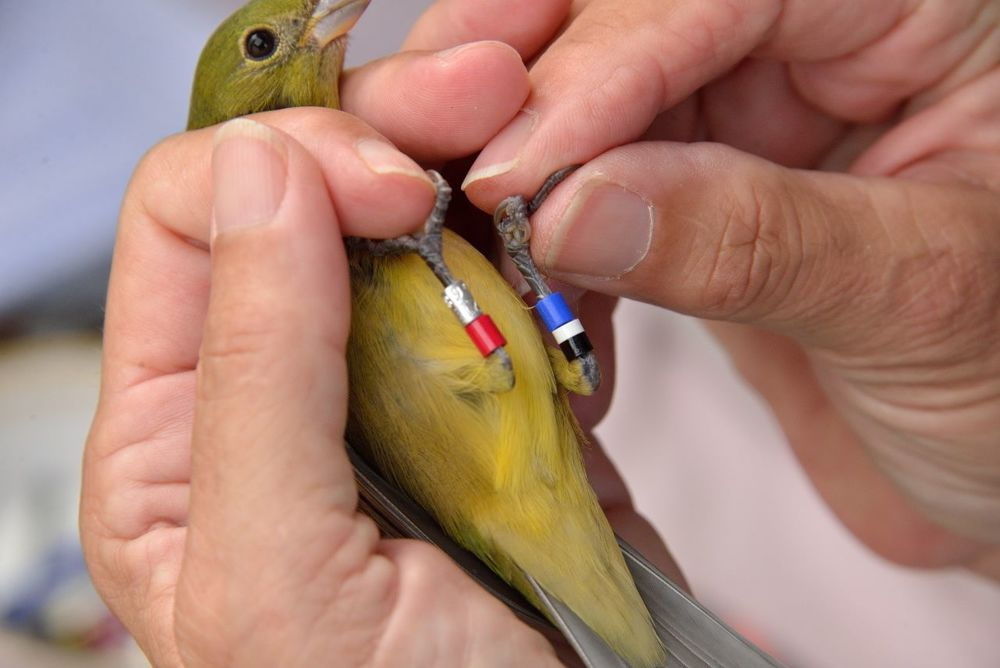
\includegraphics[width=5.14583in,height=\textheight]{Information_files/banding.png}

}

\end{figure}

\hypertarget{the-goal-of-the-question}{%
\subsection{The goal of the question}\label{the-goal-of-the-question}}

\begin{itemize}
\tightlist
\item
  learn about the data ({data summary})
\item
  apply learning outside of the data ({inference})
\item
  learn about conditions relevant to but not observed in the data
  ({prediction})
\end{itemize}

. . .

\hypertarget{inference-and-prediction}{%
\subsection{Inference and Prediction}\label{inference-and-prediction}}

\hypertarget{infernence-and-prediction}{%
\subsection{Infernence and Prediction}\label{infernence-and-prediction}}

Explanatory modeling focuses on minimizing bias to obtain the most
accurate representation of the underlying theory.

. . .

Predictive modeling focuses on minimizing both bias and estimation
variance;

. . .

this may sacrifice theoretical accuracy for improved empirical
precision.

\hypertarget{infernence-and-prediction-1}{%
\subsection{Infernence and
Prediction}\label{infernence-and-prediction-1}}

. . .

\hypertarget{statistical-information}{%
\subsection{Statistical Information}\label{statistical-information}}

Let's turn to the field of statistics to understand \emph{Information}

. . .

\href{https://en.wikipedia.org/wiki/Likelihood_principle}{Likelihood
principle}

Given a \emph{statistical model}, all the evidence/information in a
sample (\(\textbf{y}\), i.e., data) relevant to model parameters
(\(\theta\)) is contained in the \emph{likelihood function}.

. . .

\href{https://en.wikipedia.org/wiki/Fisher_information}{Fisher
Information}

The information an observable random variable (\(\textbf{y}\)) has about
an unknown parameter \(\theta\) upon which the probability of
\(\textbf{y}\) \((f(\textbf{y};\theta)\) depends.

. . .

. . .

To learn about \(\theta\) from \(\textbf{y}\), we need to link them
together via a special function, \(f(\textbf{y};\theta)\)

\hypertarget{statistical-information-1}{%
\subsection{Statistical Information}\label{statistical-information-1}}

The pieces:

\begin{itemize}
\item
  The sample data, \(\textbf{y}\)
\item
  A probability function for \(\textbf{y}\):

  \begin{itemize}
  \item
    \(f(\textbf{y};\theta)\)
  \item
    \([\textbf{y}|\theta]\)
  \end{itemize}
\item
  The unknown parameter: \(\theta\)

  \begin{itemize}
  \tightlist
  \item
    specified in the probability function
  \end{itemize}
\end{itemize}

\hypertarget{statistical-information-an-example}{%
\subsection{Statistical Information (an
example)}\label{statistical-information-an-example}}

We want to know the proportion of a wetlands that contain a rare plant
species. We can not sample the whole area.

\begin{figure}

{\centering 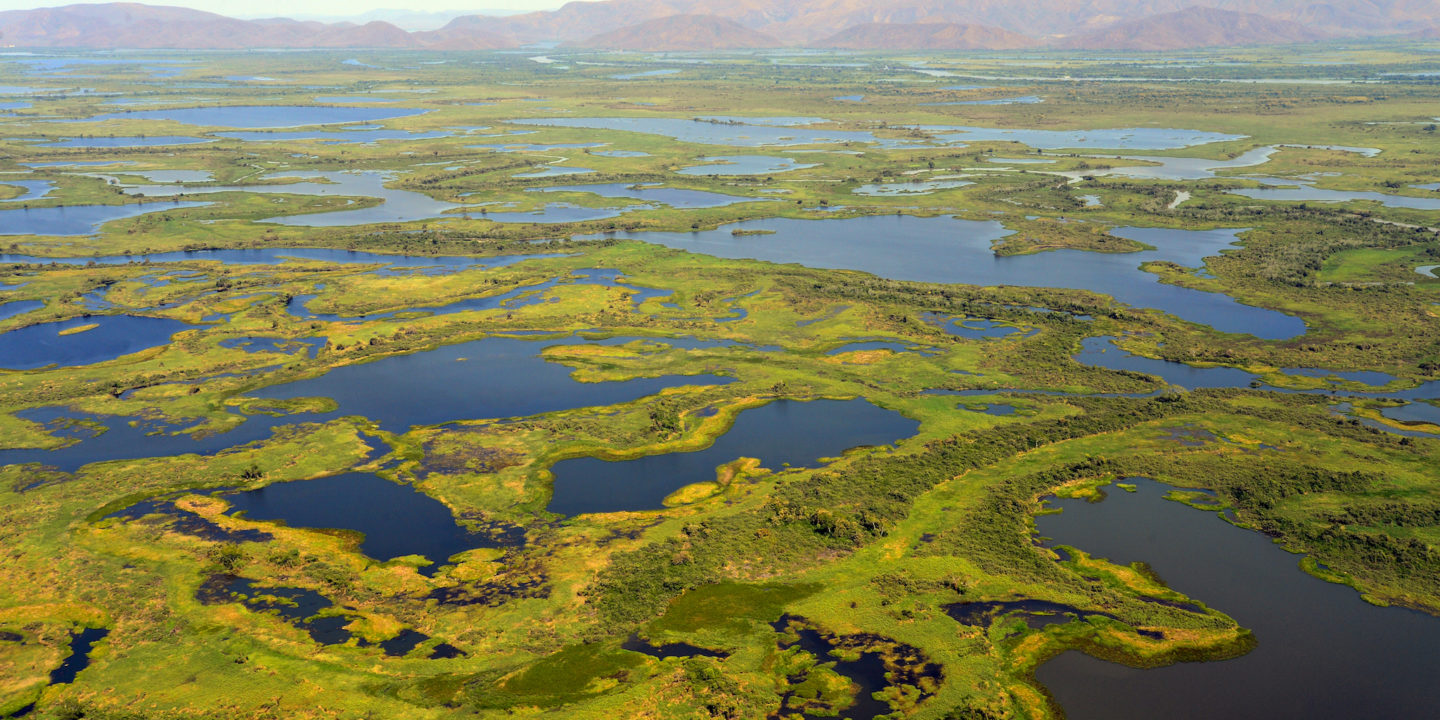
\includegraphics[width=5.14583in,height=\textheight]{Information_files/wetlands.png}

}

\end{figure}

\hypertarget{rare-plant-data}{%
\subsection{Rare Plant Data}\label{rare-plant-data}}

We randomly select plots and look for our plant.\\
Our data are

\begin{Shaded}
\begin{Highlighting}[numbers=left,,]
\NormalTok{y }\OtherTok{\textless{}{-}} \FunctionTok{c}\NormalTok{(}\DecValTok{0}\NormalTok{,}\DecValTok{1}\NormalTok{,}\DecValTok{1}\NormalTok{,}\DecValTok{1}\NormalTok{,}\DecValTok{1}\NormalTok{,}\DecValTok{0}\NormalTok{,}\DecValTok{1}\NormalTok{,}\DecValTok{0}\NormalTok{,}\DecValTok{0}\NormalTok{,}\DecValTok{0}\NormalTok{)}
\NormalTok{n }\OtherTok{\textless{}{-}} \FunctionTok{length}\NormalTok{(y)}
\NormalTok{n}
\end{Highlighting}
\end{Shaded}

\begin{verbatim}
[1] 10
\end{verbatim}

. . .

\(\textbf{y}\) is a random variable as it depends on random events.

. . .

In this case, when we induced a random selection of sites.

\hypertarget{probabilitylikelihood-function}{%
\subsection{Probability/Likelihood
Function}\label{probabilitylikelihood-function}}

\(f(\textbf{y};\theta)\) describes the probability for each \(i^{th}\)
data, \(y_i\).

But, not just for the data we observed, for all possible data that could
be observed.

. . .

\textbf{Rules about our data:} \(y \in \{0,1\}\),

. . .

. . .

\textbf{Not this:} \(y \in [0,1]\),

. . .

\textbf{Not this:} \(y \in (0,1)\),

\hypertarget{probability-function}{%
\subsection{Probability Function}\label{probability-function}}

Two outcomes, 0 or 1, so we need two probabilities to describe our
random variable.

. . .

\[
  f(y;\theta) = [y|\theta]= 
  \begin{cases}
    \theta     & \text{if $y = 1$}, \\
    1 - \theta & \text{if $y = 0$}.
  \end{cases}
\]

. . .

Also,

\[
f(y;\theta) = [y|\theta]=
  \begin{align}
        \theta^{y}\times(1-\theta)^{1-y}
  \end{align}
\]

. . .

Also,

\[
  \begin{align}
        P(Y=1) &= \theta \\
        P(Y=0) &= 1-\theta  
  \end{align}
\]

\hypertarget{probability-function-1}{%
\subsection{Probability Function}\label{probability-function-1}}

Probabilities, such as our parameter, have rules:

\begin{itemize}
\item
  \(0 \leq \theta \leq 1\)
\item
  \(0 \leq (1 - \theta) \leq 1\)
\item
  \(\theta + (1-\theta) = 1\)
\end{itemize}

\hypertarget{probability-function-2}{%
\subsection{Probability Function}\label{probability-function-2}}

How do we find \(\theta\) for our data?

. . .

We can use our probability function to calculate the likelihood of a
parameter, given our data.

. . .

\[
\mathcal{L}(\theta|y) = \prod_{i=1}^{n} p(y_{i};\theta)
\]

. . .

\begin{Shaded}
\begin{Highlighting}[numbers=left,,]
\CommentTok{\#Bernoulli probability function}
\NormalTok{  prob.function}\OtherTok{=}\ControlFlowTok{function}\NormalTok{(theta)\{}\FunctionTok{prod}\NormalTok{(theta}\SpecialCharTok{\^{}}\NormalTok{y}\SpecialCharTok{*}\NormalTok{(}\DecValTok{1}\SpecialCharTok{{-}}\NormalTok{theta)}\SpecialCharTok{\^{}}\NormalTok{y)\}}

\CommentTok{\#possible probabilities}
\NormalTok{  theta.guess}\OtherTok{=}\FunctionTok{matrix}\NormalTok{(}\FunctionTok{seq}\NormalTok{(}\FloatTok{0.01}\NormalTok{,}\FloatTok{0.99}\NormalTok{,}\AttributeTok{by=}\FloatTok{0.01}\NormalTok{))}

\CommentTok{\#implement function}
\NormalTok{  likelihood}\OtherTok{=}\FunctionTok{apply}\NormalTok{(theta.guess,}\DecValTok{1}\NormalTok{,prob.function)}
  
\CommentTok{\#Find maximum likelood}
\NormalTok{  max.index}\OtherTok{=}\FunctionTok{which.max}\NormalTok{(likelihood)}

\CommentTok{\#Theta that maximizes our probability function}
\NormalTok{  theta.est}\OtherTok{=}\NormalTok{theta.guess[max.index]}

\CommentTok{\#Define other probability}
\NormalTok{  q.est }\OtherTok{\textless{}{-}} \DecValTok{1}\SpecialCharTok{{-}}\NormalTok{theta.est}

\CommentTok{\#Alternative estimation}
\NormalTok{  theta.est2 }\OtherTok{\textless{}{-}} \FunctionTok{sum}\NormalTok{(y)}\SpecialCharTok{/}\NormalTok{n}
\end{Highlighting}
\end{Shaded}

. . .


\includegraphics{Information_files/figure-pdf/unnamed-chunk-3-1.pdf}

\hypertarget{statistical-information-an-example-1}{%
\subsection{Statistical Information (an
example)}\label{statistical-information-an-example-1}}

Let's combine 1 observation of our random variable, our probability
function, and \(\theta\) to quantify the Fisher information
(\href{https://en.wikipedia.org/wiki/Fisher_information\#Single-parameter_Bernoulli_experiment}{Link}
):

. . .

\begin{align}
I(\theta) &= -E\left[\frac{\partial^2}{\partial\theta^2}\text{log}(\theta^y(1-\theta)^{1-y}) \right]\\
\end{align}

. . .

For all samples (n), this is reduced to

\begin{align}
I(\theta) &= \frac{n}{\theta(1-\theta)}\\
\end{align}

\hypertarget{statistical-information-an-example-2}{%
\subsection{Statistical Information (an
example)}\label{statistical-information-an-example-2}}

Therefore, for our sample

\begin{Shaded}
\begin{Highlighting}[]
\NormalTok{I }\OtherTok{=}\NormalTok{ n}\SpecialCharTok{/}\NormalTok{(theta.est}\SpecialCharTok{*}\NormalTok{q.est)}
\NormalTok{I}
\end{Highlighting}
\end{Shaded}

\begin{verbatim}
[1] 40
\end{verbatim}

. . .

Consider how information varies by \(\theta\) for a given sample
size\ldots.

\hypertarget{statistical-information-an-example-3}{%
\subsection{Statistical Information (an
example)}\label{statistical-information-an-example-3}}

\begin{Shaded}
\begin{Highlighting}[numbers=left,,]
\NormalTok{thetas}\OtherTok{=}\FunctionTok{seq}\NormalTok{(}\FloatTok{0.05}\NormalTok{,}\FloatTok{0.95}\NormalTok{,}\FloatTok{0.1}\NormalTok{)}

\NormalTok{Information }\OtherTok{\textless{}{-}}\NormalTok{ n}\SpecialCharTok{/}\NormalTok{(thetas}\SpecialCharTok{*}\NormalTok{(}\DecValTok{1}\SpecialCharTok{{-}}\NormalTok{thetas))}

\FunctionTok{par}\NormalTok{(}\AttributeTok{cex.lab=}\FloatTok{2.5}\NormalTok{,}\AttributeTok{cex.axis=}\FloatTok{2.5}\NormalTok{,}\AttributeTok{mar=}\FunctionTok{c}\NormalTok{(}\DecValTok{5}\NormalTok{,}\DecValTok{5}\NormalTok{,}\DecValTok{2}\NormalTok{,}\DecValTok{2}\NormalTok{))}
\FunctionTok{plot}\NormalTok{(thetas,Information,}\AttributeTok{type=}\StringTok{"b"}\NormalTok{,}\AttributeTok{lwd=}\DecValTok{8}\NormalTok{)}

\FunctionTok{abline}\NormalTok{(}\AttributeTok{v=}\NormalTok{theta.est,}\AttributeTok{col=}\DecValTok{2}\NormalTok{,}\AttributeTok{lwd=}\DecValTok{8}\NormalTok{)}
\end{Highlighting}
\end{Shaded}

\begin{figure}[H]

{\centering 
\includegraphics{Information_files/figure-pdf/unnamed-chunk-5-1.pdf}

}

\end{figure}

\hypertarget{statistical-information-an-example-4}{%
\subsection{Statistical Information (an
example)}\label{statistical-information-an-example-4}}

Funny enough, Fisher Information is the reciprocal of the variance of
our estimate of
\(\theta\),\[Var[\hat{\theta}] = \frac{\hat{\theta}  (1-\hat{\theta})}{n}\]

\hypertarget{statistical-information-an-example-5}{%
\subsection{Statistical Information (an
example)}\label{statistical-information-an-example-5}}

\begin{Shaded}
\begin{Highlighting}[numbers=left,,]
\NormalTok{thetas}\OtherTok{=}\FunctionTok{seq}\NormalTok{(}\FloatTok{0.05}\NormalTok{,}\FloatTok{0.95}\NormalTok{,}\FloatTok{0.1}\NormalTok{)}

\NormalTok{Var.theta }\OtherTok{\textless{}{-}}\NormalTok{ (thetas}\SpecialCharTok{*}\NormalTok{(}\DecValTok{1}\SpecialCharTok{{-}}\NormalTok{thetas))}\SpecialCharTok{/}\NormalTok{n}
\FunctionTok{par}\NormalTok{(}\AttributeTok{cex.main=}\FloatTok{2.5}\NormalTok{,}\AttributeTok{cex.axis=}\FloatTok{2.5}\NormalTok{,}\AttributeTok{cex.lab=}\FloatTok{2.5}\NormalTok{,}\AttributeTok{mar=}\FunctionTok{c}\NormalTok{(}\DecValTok{5}\NormalTok{,}\DecValTok{5}\NormalTok{,}\DecValTok{2}\NormalTok{,}\DecValTok{2}\NormalTok{))}
\FunctionTok{plot}\NormalTok{(thetas,Var.theta,}\AttributeTok{type=}\StringTok{"b"}\NormalTok{,}\AttributeTok{lwd=}\DecValTok{8}\NormalTok{)}
\FunctionTok{abline}\NormalTok{(}\AttributeTok{v=}\NormalTok{theta.est,}\AttributeTok{col=}\DecValTok{2}\NormalTok{,}\AttributeTok{lwd=}\DecValTok{8}\NormalTok{)}
\end{Highlighting}
\end{Shaded}

\begin{figure}[H]

{\centering 
\includegraphics{Information_files/figure-pdf/unnamed-chunk-6-1.pdf}

}

\end{figure}

. . .

How does this knowledge about this probability function inform the
design of a study?

\hypertarget{statistics}{%
\subsection{Statistics}\label{statistics}}

A field dedicated to observing the real world to gain informational
data.

. . .

Often statistics classes only focus on Power Analysis.

. . .

\begin{itemize}
\tightlist
\item
  how our data will be created
\item
  our question of the data
\item
  a probability function to use and its parameters
\item
  the goal of the question
\end{itemize}

\hypertarget{reading}{%
\subsection{Reading}\label{reading}}

\begin{figure}

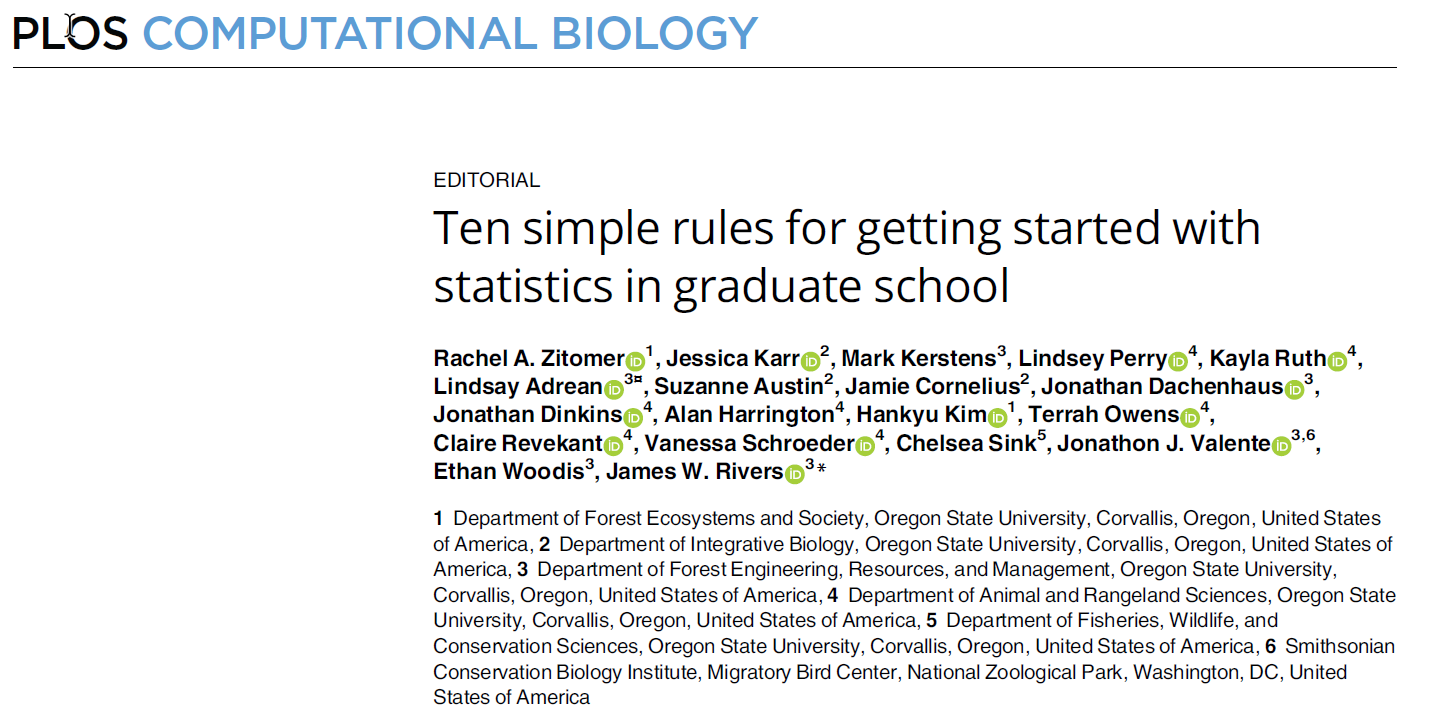
\includegraphics[width=10.41667in,height=\textheight]{Information_files/reading0.png} \hfill{}

\end{figure}

\href{https://journals.plos.org/ploscompbiol/article?id=10.1371/journal.pcbi.1010033}{Link}



\end{document}
